\def\CTeXPreproc{Created by ctex v0.2.9, don't edit!}
%\documentclass{beamer}
\documentclass[%handout,
xcolor=pdftex]{beamer}
\mode<presentation> {
  \usetheme{Warsaw}
  \setbeamercovered{transparent}
}
\let\Tiny=\tiny
\usetheme{Singapore}
\usecolortheme{dolphin}
\usepackage{amsmath}
\usepackage{textcomp}
\usepackage{amssymb}
\usepackage{amsthm}
\usepackage{graphicx}
\usepackage{color}
\usepackage{lipsum}
\usepackage{hyperref}
\usepackage{multirow}
\usepackage{bm}
%\setbeamertemplate{headline}{}
\setbeamertemplate{footline}[page number]
\newcommand\Fontvi{\fontsize{9pt}{8}\selectfont}
\newcommand\Fontvii{\fontsize{7pt}{8}\selectfont}
\newcommand{\backupbegin}{
   \newcounter{finalframe}
   \setcounter{finalframe}{\value{framenumber}}
}
\newcommand{\backupend}{
   \setcounter{framenumber}{\value{finalframe}}
}\newtheorem{proposition}{Proposition}
\title{Unit 7: Smoothing}
\author[STAT 5170: Applied Time Series, Unit 6]{Taylor R. Brown PhD}
\institute{Department of Statistics, University of Virginia}
\date{Spring 2020}

\AtBeginSubsection[] {
  \begin{frame}<beamer>{Outline}
    \tableofcontents[currentsection,currentsubsection]
  \end{frame}
}

\begin{document}


\frame{\titlepage}


\begin{frame}
\frametitle{Readings for Unit 7}

Textbook chapter 2.3.

\end{frame}


\begin{frame}
\frametitle{Last Unit}
\begin{enumerate}
\item Periodic functions
\item Exploratory data tools to access frequency
\end{enumerate}
\end{frame}

\begin{frame}
\frametitle{This Unit}
Smoothing techniques:
\begin{enumerate}
\item Averaging
\item Kernel Smoothing
\item Nearest Neighbors Regression
\end{enumerate}
\end{frame}

\begin{frame}
\frametitle{Motivation}

Sometimes, the time series data we have can be too noisy to be able to detect long term trends. Smoothing is used to smooth out short term random fluctuations so that longer term trends can be emphasized.

\end{frame}

\section{Averaging}
\frame{\tableofcontents[currentsection]}

\begin{frame}
\frametitle{So Far...}

So far, we have looked to fit models of the form
$$
x_t=\mu_t +y_t
$$
where $\mu_t$ is a function and $y_t$ is stationary.  We've already discussed when $\mu_t$ is of the form
$$
\beta_0+\beta_1 t+...+\beta_{p} t^p
$$
or
$$
\beta_1 cos(2 \pi \omega  t)+\beta_2 sin(2 \pi \omega  t).
$$

% In the context of smoothing, we will denote $\mu_t$ by $\mu_t$.

\end{frame}

\begin{frame}
\frametitle{Averaging}

One way to approximate $\mu_t$ is to take a moving average of the time series.  Averaging, in general, \textbf{reduces variability}.  It can also reduce ``seasonal'' fluctuations. Averaging can help in viewing \textbf{longer term trends}, because the seasonal variations will be dampened.  In general we may write a moving average as

\begin{equation} \label{eq:avg}
m_t=\sum_{j=-k}^{k} a_j x_{t-j},
\end{equation}

where $a_j \geq 0$ and $\sum_{j=-k}^k a_j = 1$.

\end{frame}

\begin{frame}
\frametitle{Averaging}

Equation (\ref{eq:avg}) can be used as an estimate of $\mu_t$. The smoothed value for a particular time is calculated as a \textbf{linear combination} of observations for surrounding times. \\
\vspace{5mm}
Equation (\ref{eq:avg}) is sometimes also called a centered moving average, since we average with $k$ times before and $k$ times after. For example, a centered moving average of length 5 with equal weights would be the average of values at times $t-2, t-1, t, t+1, t+2$.

\end{frame}

\begin{frame}
\frametitle{Averaging}

Smoothing using (\ref{eq:avg}) has the advantage of being adaptable to slow changes in $\mu_t$ across time.  The disadvantage is that there may still be a substantial amount of variability in our estimate $\mu_t$, and we may not know {\bf a priori} what the window size, $k$, should be.  With some data, there will be a natural window size; with others there may not be.

\end{frame}

\begin{frame}
\frametitle{Window Size}

\textbf{Question:} What is an appropriate window size, $k$, to smooth away seasonality in quarterly data, in order to identify yearly trends? What about monthly data? 


\vspace{50mm}



\end{frame}


\begin{frame}
\frametitle{Variance Reduction with Averaging}

It was mentioned earlier that averaging reduces variation, in general. Let's look at an example. Assume that the original series $x_t$  is
stationary, such that $V(x_t) = \sigma^2$. Let's create another time series
$$
y_t=\frac{1}{3} x_{t+1}+\frac{1}{3} x_{t}+\frac{1}{3} x_{t-1}.
$$

\textbf{Question:} Derive the variance of $y_t$.

\end{frame}

\begin{frame}
\frametitle{Variance Reduction with Averaging}


\end{frame}

\begin{frame}
\frametitle{Example: Cardiovascular Mortality in Los Angeles}

In this example, we look at the weekly cardiovascular mortality in Los Angeles county. We have a plot of the data below.

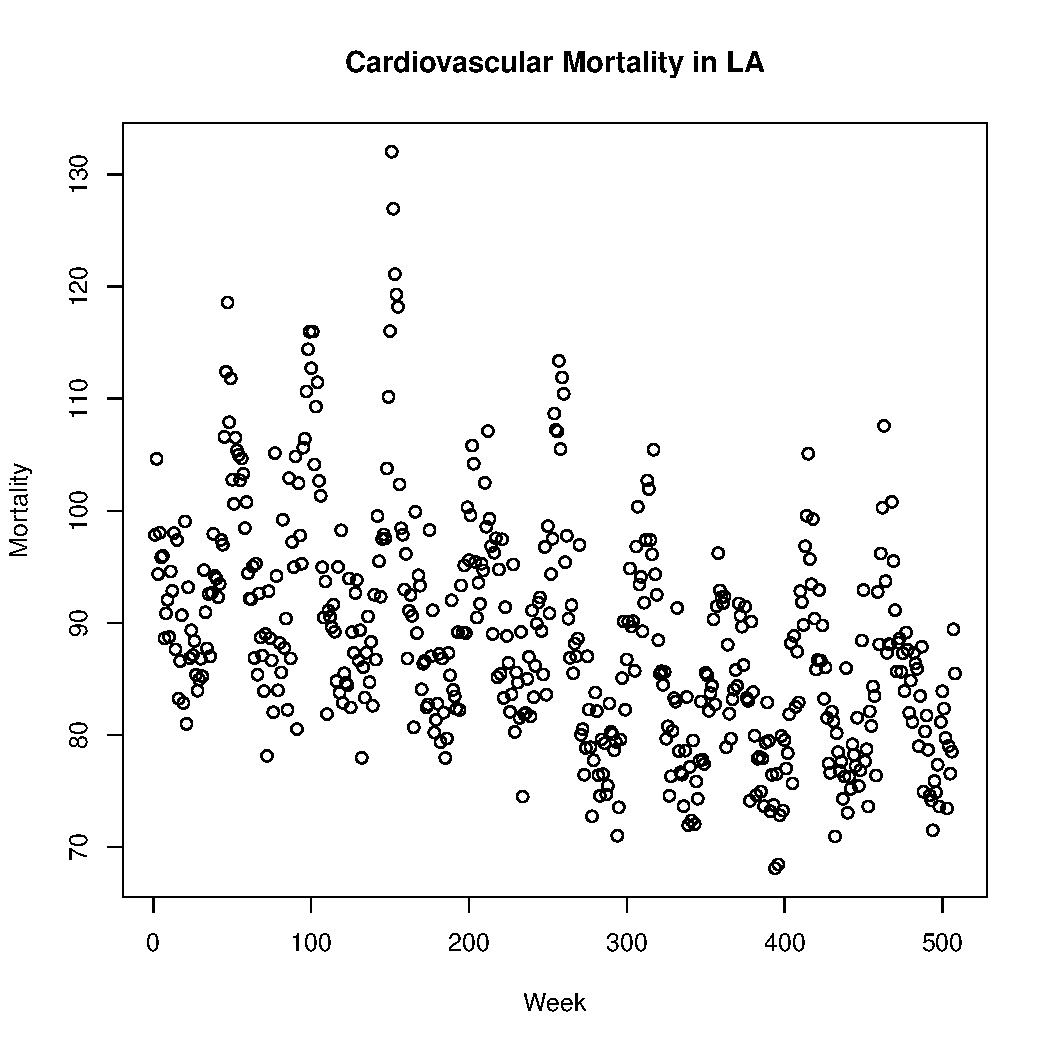
\includegraphics[width=100mm, height=60mm]{mort.pdf}

Comments on seasonal trend? Yearly trend?

\end{frame}



\begin{frame}
\frametitle{Example: Cardiovascular Mortality in Los Angeles}

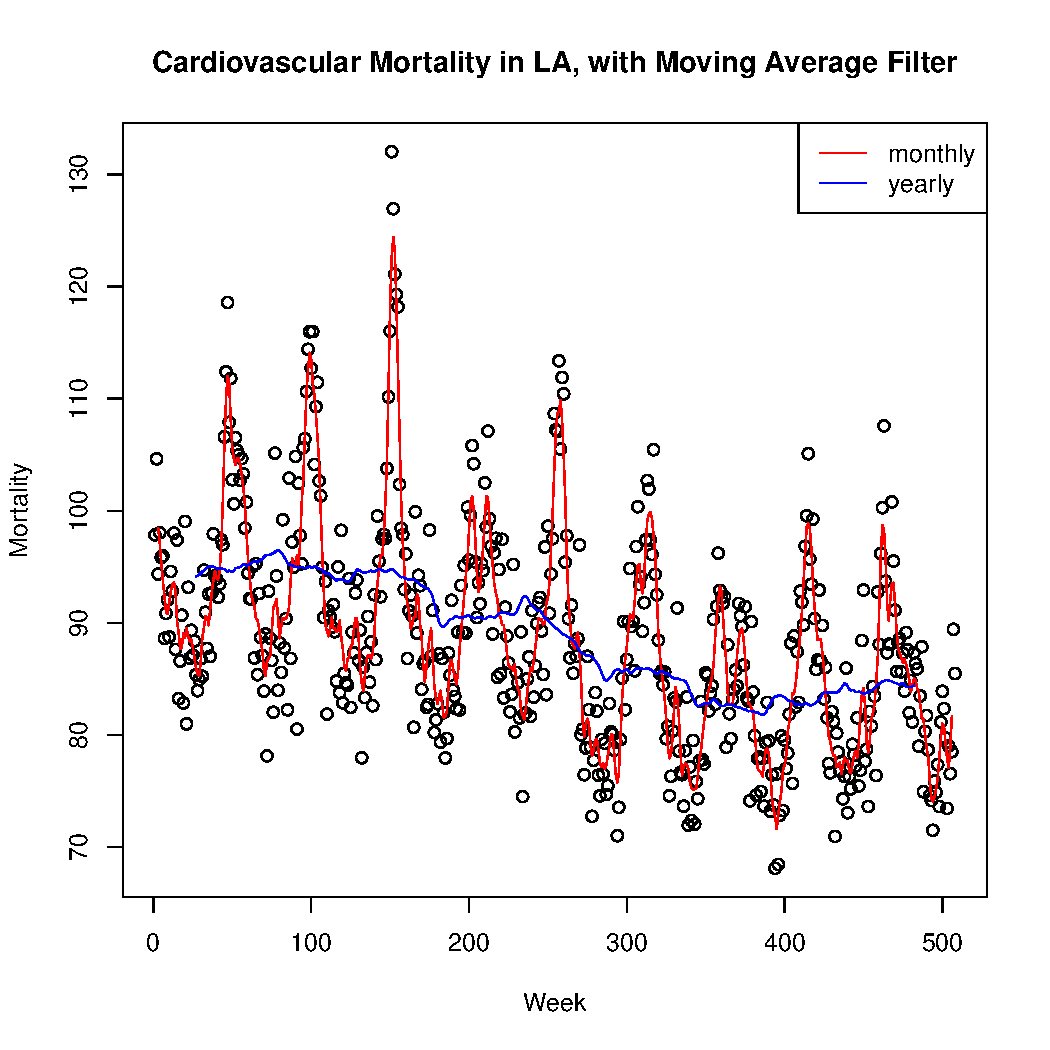
\includegraphics[width=100mm, height=60mm]{filter.pdf}

Comments on monthly and/or yearly trend?

\end{frame}

\begin{frame}
\frametitle{Example: Cardiovascular Mortality in Los Angeles}

Due to the symmetric nature of the moving average, we will be taking the weighted average of an odd number of observations. To detect monthly trends using weekly data, we'd like to take the weighted average of four weeks. One way to work around this is to consider weights

$$
a_0 = a_{\pm1} = 1/4, a_{\pm2} = 1/8,
$$

with $k=2$. \textbf{Question:} what weights should we use to detect yearly trends for this series?

\end{frame}

\begin{frame}[fragile]
\frametitle{Example: Cardiovascular Mortality in Los Angeles}

\begin{verbatim}
plot(mort)
ma4<-filter(mort,sides=2,c(0.5, rep(1,3), 0.5)/4)
ma52<-filter(mort,sides=2,c(0.5, rep(1,51), 0.5)/52)
lines(ma4, col="red")
lines(ma52, col="blue")
\end{verbatim}

\end{frame}

\section{Kernel Smoothing}
\frame{\tableofcontents[currentsection]}

\begin{frame}
\frametitle{Kernel Smoothing}

%There are a number of other methods to smooth a time series.  One popular method is kernel smoothing.
The idea with kernel smoothing is similar to the moving average; however, the contribution to the estimate of the smooth function at a point $t$ from local points declines as a function of distance from the current point.  The smooth function is estimated by
\begin{equation}
\hat{\mu_t}=\sum_{i=1}^n w_t(i) x_j
\end{equation}
where

\begin{equation} \label{eq:weight}
w_t(i)=\frac{K\left( \frac{t-i}{b} \right)}{ \sum_{i=1}^n K\left( \frac{t-i}{b} \right)}.
\end{equation}

In (\ref{eq:weight}), $K(.)$ is the \textbf{kernel function}, and $b$ is the \textbf{bandwidth}.

\end{frame}

\begin{frame}
\frametitle{Kernel Smoothing}

A common choice for $K(.)$ is a standard normal density; in this case, $K(z) = \frac{1}{\sqrt{2\pi}} \exp(-z^2/2)$.  Other choices include the uniform density. \\

\vspace{5mm}

An issue with kernel smoothing is the choice of $b$.  This will help determine how much of $\mu_t$ is determined by neighboring points. The \textbf{wider} the bandwidth, the smoother the result.

\end{frame}

\begin{frame}
\frametitle{Example: Cardiovascular Mortality in Los Angeles}

We apply normal kernel smoothing to the cardiovascular data.

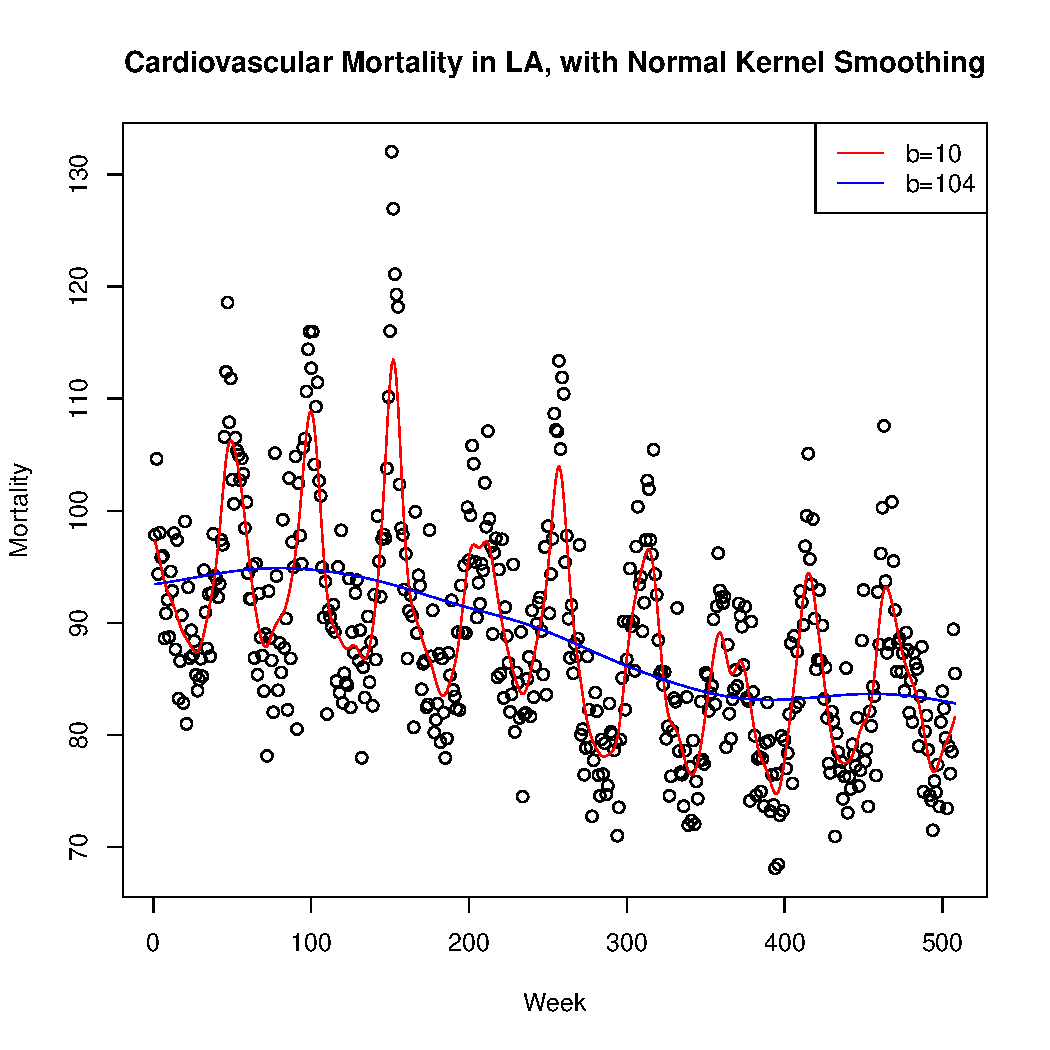
\includegraphics[width=100mm, height=60mm]{kernel_normal.pdf}

\end{frame}

\begin{frame}
\frametitle{Example: Cardiovascular Mortality in Los Angeles}

We apply uniform kernel smoothing to the cardiovascular data.

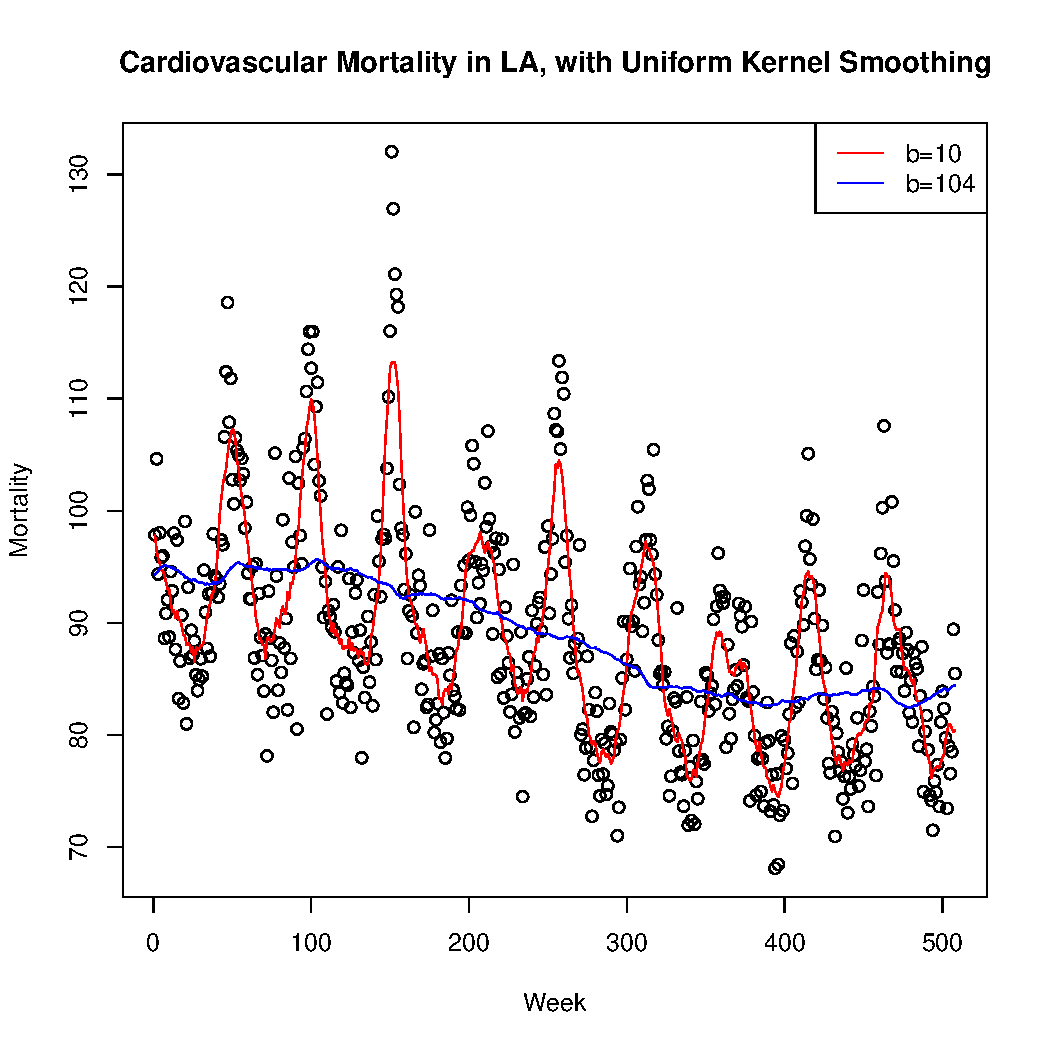
\includegraphics[width=100mm, height=60mm]{kernel_u.pdf}

\end{frame}

\begin{frame}[fragile]
\frametitle{Example: Cardiovascular Mortality in Los Angeles}

\begin{verbatim}
t<-1:length(mort)
plot(t,mort)
lines(ksmooth(t,mort, "normal", bandwidth=10))
lines(ksmooth(t,mort, "normal", bandwidth=104))
\end{verbatim}

\end{frame}

\section{Nearest Neighbors Regression}
\frame{\tableofcontents[currentsection]}

\begin{frame}
\frametitle{Nearest Neighbors Regression}

Another technique is nearest neighbors regression. This is based on $k$-nearest linear regression, where $\{x_{t-k/2}, \cdots, x_t, \cdots, x_{t+k/2} \}$ to predict $x_t$ via linear regression.

\end{frame}

\begin{frame}
\frametitle{Example: Cardiovascular Mortality in Los Angeles}

We apply nearest neighbors regression to the cardiovascular data.

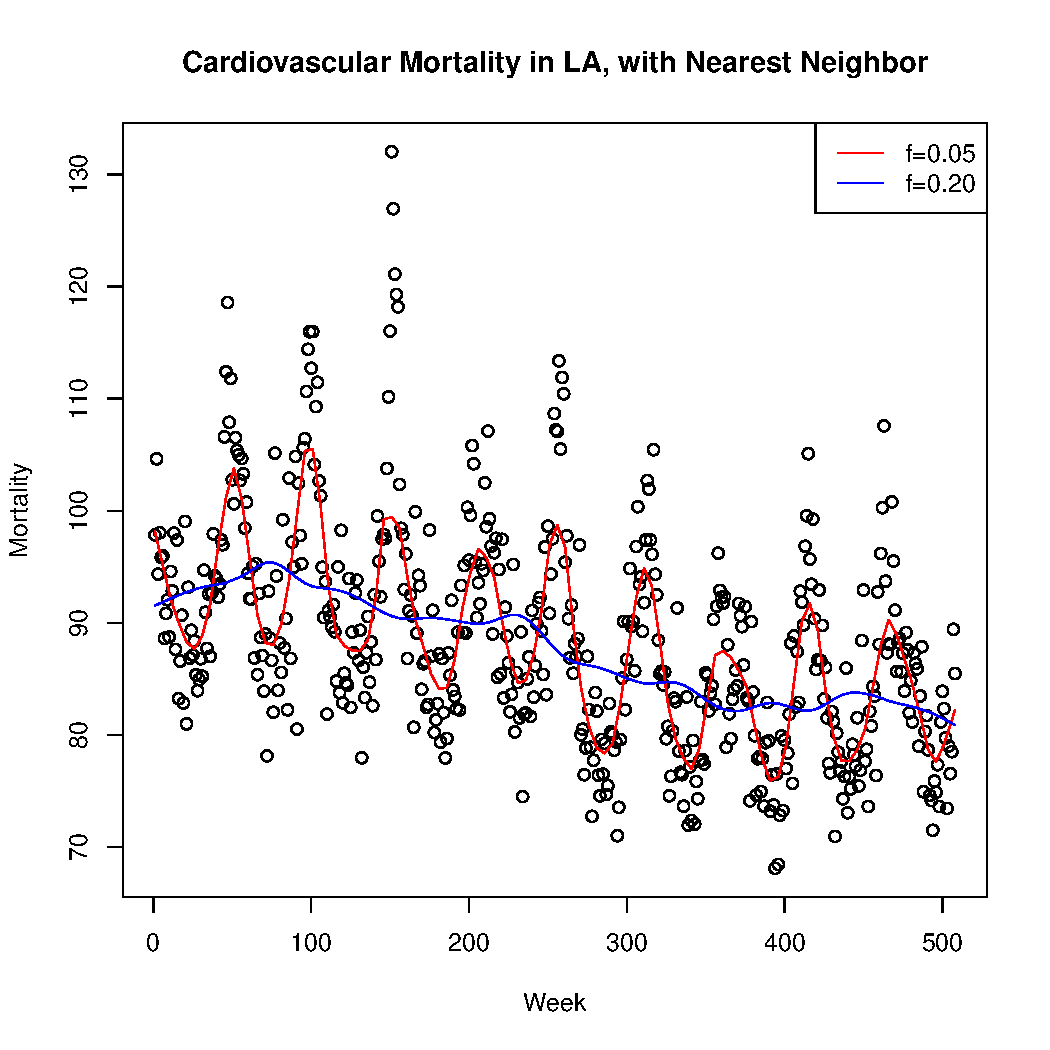
\includegraphics[width=100mm, height=60mm]{neighbor.pdf}

\end{frame}

\begin{frame}[fragile]
\frametitle{Example: Cardiovascular Mortality in Los Angeles}

\begin{verbatim}
plot(t,mort)
lines(lowess(t,mort,f=0.05),col="red")
lines(lowess(t,mort,f=0.20),col="blue")
\end{verbatim}

\end{frame}

\begin{frame}
\frametitle{Under-smoothing Vs Over-smoothing}

\textbf{Question}: What are the consequences of under-smoothing and over-smoothing?

\end{frame}

\begin{frame}
\frametitle{Summary}

It can be difficult to detect trends and patterns in time series plots. Smoothing can help us dampen irregularities so we get a clearer idea on the time series. Note that all of the techniques discussed can be used, however, the most important aspect in using them is knowing the right parameters to use (e.g. bandwith, window etc.) These techniques aid us in develop an appropriate model for our data and should be used as a guide.

\end{frame}

\end{document} 